\documentclass[upright, contnum]{umemoria}

%fix for the oneside argument
\makeatletter
\g@addto@macro\titlepage{\pagenumbering{Alph}}
\g@addto@macro\endtitlepage{\pagenumbering{roman}}
\makeatother

\depto{Departamento de Ciencias de la Computación}
\author{Matías Ignacio Meneses Cortés}
\title{Type-Based Declassification en Dart: Implementación y Elaboración de Herramientas de Inferencia}
\auspicio{}
\date{Abril 2018}
\guia{Éric Tanter}
\carrera{Ingeniero Civil en Computación}
\memoria{Memoria para optar al Título de \break  Ingeniero Civil en Computación}
\comision{}

\usepackage{lipsum}
\usepackage{tikz}
\usetikzlibrary{positioning}
\usepackage[utf8]{inputenc}
\usepackage[T1]{fontenc}
\usepackage{color}
\usepackage{proof}
\usepackage{caption}
\usepackage{algorithm, algpseudocode}
\makeatletter
\renewcommand{\ALG@name}{Algoritmo}
\renewcommand{\ALG@beginalgorithmic}{\small}
\makeatother

% New definitions
\algnewcommand\algorithmicswitch{\textbf{switch}}
\algnewcommand\algorithmiccase{\textbf{case}}
\algnewcommand\algorithmicassert{\texttt{assert}}
\algnewcommand\Assert[1]{\State \algorithmicassert(#1)}%
% New "environments"
\algdef{SE}[SWITCH]{Switch}{EndSwitch}[1]{\algorithmicswitch\ #1\ \algorithmicdo}{\algorithmicend\ \algorithmicswitch}%
\algdef{SE}[CASE]{Case}{EndCase}[1]{\algorithmiccase\ #1}{\algorithmicend\ \algorithmiccase}%
\algtext*{EndSwitch}%
\algtext*{EndCase}%

\definecolor{dkgreen}{rgb}{0,0.6,0}
\definecolor{gray}{rgb}{0.5,0.5,0.5}
\definecolor{mauve}{rgb}{0.58,0,0.82}

\usepackage{listings}
\lstset{%
	numberstyle=\tiny,
	numbersep=15pt,tabsize=4,
	flexiblecolumns=true,
	keywordstyle=\color{blue},
	commentstyle=\color{dkgreen},
	stringstyle=\color{mauve},
	numberstyle=\tiny\color{gray},
	language=Java,
	breaklines=true,
	breakatwhitespace=true,
  showstringspaces=false,
  aboveskip=1.2em,
  belowskip=1.2em,
	morekeywords={*,num,String,var,library,get,set,StringEq,bool,Top,Bot,<} ,
}

\begin{document}
\setcounter{chapter}{1}
\frontmatter
\maketitle

\begin{abstract}
{\lipsum[1-1]}
\end{abstract}

\begin{dedicatoria} % opcional
Una dedicatoria corta. Por ejemplo, \emph{A los creadores de U-Campus}
\end{dedicatoria}

\begin{thanks} % opcional
\lipsum[1-2]
\end{thanks}
\cleardoublepage

\tableofcontents
\listoftables % opcional
\listoffigures % opcional

\mainmatter



\begin{intro}

	La protección de la confidencialidad de la información manipulada por los programas computacionales es un problema cuya relevancia se ha incrementado en el último tiempo, a pesar de tener varias décadas de investigación. Por ejemplo, una aplicación web (o móvil) que como parte de su funcionamiento debe interactuar con servicios de terceros y por tanto debe proteger que su información sensible no se escape durante la ejecución de la aplicación a canales públicos.

	Muchas de las técnicas de seguridad convencionales como \textit{control de acceso} tienen deficiencias para proteger la confidencialidad de un programa, por ejemplo no restringen la propagación de información\cite{myers-phd}.

	Formas más expresivas y efectivas de proteger la confidencialidad se basan en un análisis estático sobre el código del programa, y se categorizan dentro de \textit{language-based security}. Una de las técnicas más efectivas se denomina \textit{tipado de seguridad} en un \textit{lenguaje de seguridad}, donde los tipos son anotados con niveles de seguridad para clasificar la información manipulada por el programa.

	Uno de los mayores desafíos de los lenguajes de seguridad es facilitar el trabajo del programador, utilizando técnicas más expresivas. En esta dirección, Cruz et al.~\cite{cruzAl:ecoop2017} recientemente propusieron \textit{type-based declassification}, una variación de tipado de seguridad que utiliza el sistema de tipos del lenguaje para controlar la declasificación de la información.

	\textit{Type-based declassification} presenta limitaciones en cuanto a su implementación, debido a que el análisis teórico se realiza sobre un lenguaje minimalista que no incluye características básicas de los lenguajes de programación, como instrucciones condicionales y mutabilidad. En este trabajo, se propone una extensión al lenguaje minimalista utilizado en \textit{type-based declassification}, y la implementación en el lenguaje de programación Dart, desarrollando un plugin para los editores de texto más populares, con el objetivo de proporcionar una experiencia interactiva e intuitiva al usuario.



		\section{Motivación}
	El tema escogido se considera interesante debido a su importancia teórica y práctica en el campo de la seguridad en lenguajes de programación. Los fundamentos teorícos de \textit{type-based declassification} están bien descritos~\cite{cruzAl:ecoop2017}, pero no así su realización práctica, siendo esto reconocido por sus autores.

	Se considera que la realización de este trabajo es relevante para demostrar y materializar en un lenguaje de uso general la investigación de type-based declassification. Dicha materalización constituye un desafío importante en términos de complejidad, al tener que entender la teoría subyacente de tipado de seguridad, así como extender un lenguaje real y sus herramientas de análisis estático con nuevas funcionalidades.

		\section{Objetivos}
	El objetivo de la memoria es realizar la implementación de un sistema de inferencia para \textit{type-based declassification}. Dentro de los objetivos específicos del trabajo, podemos encontrar:

	\begin{itemize}
	\item \textbf{Inferencia y verificación estática de type-based declassification}. Se entiende coma la implementación de un sistema de inferencia de facetas de declasificación para \textit{type-based declassification}, en el lenguaje de programación Dart. Dentro del análisis de la inferencia se incluye la verificación de las reglas del sistema de tipos de \textit{type-based declassification}.

	\item \textbf{Plugin para editores}. Mostrar al programador el resultado de la inferencia, por medio de un plugin para los editores de texto que soporten servidores de análisis estático de Dart, ofreciéndole acciones al respecto.

	\end{itemize}

		\section{Resultados y Organización del documento}

	En términos concretos este trabajo presenta el diseño de un plugin que realiza el análisis de type-based declassification. Los antecedentes teóricos necesarios para entender este trabajo se abordan en el capítulo 2, mientras que la propuesta de solución es desarrollada en el capítulo 3.

	Los detalles de diseño de implementación de la propuesta son revisados en el capítulo 4.

	% TODO
	Por terminar.


\end{intro}

\chapter{Control de flujo de información} \label{controlflujo}
El control de flujo de información es una técnica de seguridad que permite controlar las acciones que se pueden realizar con los valores que manipula un programa, y hacia dónde está permitido que fluyan. En este capítulo se presentan los antecedentes de tipado de seguridad para el control de flujo de información, y los conceptos importantes de la desclasificación basada en tipos.

\section{Tipado de seguridad}
Los lenguajes con tipado de seguridad para el control del flujo de la información clasifican los valores de un programa con respecto a sus niveles de confidencialidad, expresado mediante un retículo\footnote{Un orden parcial, donde todo par de elementos tiene un único supremo e ínfimo} (\emph{lattice}) de etiquetas de seguridad. Por ejemplo, con el retículo de dos niveles de seguridad \texttt{L} $\sqsubseteq$ \texttt{H} se puede distinguir entre valores públicos o de baja confidencialidad (\texttt{L}) y valores privados o de alta confidencialidad (\texttt{H}). Un sistema de tipos con control de flujo asegura de forma estática el cumplimiento de la propiedad de no-interferencia~\cite{noninterference}, esto es, que la información confidencial no fluya directa o indirectamente hacia canales públicos~\cite{volpanoAl:S96}.

A modo de ejemplo, consideremos una aplicación móvil que permite encontrar un hotel cercano utilizando Google Maps, y luego reservar una habitación en ese hotel ingresando los datos de la tarjeta de crédito. La información confidencial involucrada en este caso son los datos de la tarjeta de crédito, que deben ser enviados al hotel para realizar la reserva. En el ejemplo \ref{ej2-1} se muestra el código de una función \texttt{book} que realiza la reserva, y las funciones \texttt{sendToHotel} y \texttt{sendToGoogleMaps} que envían información a los respectivos servicios.
\clearpage
\begin{ej} \ \\
  \normalfont
  \label{ej2-1}
\begin{lstlisting}
  String book(String username, int date, int cardNumber) {
    return sendToHotel(username, date, cardNumber);
  }

  String sendToHotel(String username, int date, int cardNumber);
  String sendToGoogleMaps(String token, int xCoord, int yCoord);
\end{lstlisting}
\end{ej}

La función \texttt{book} del ejemplo \ref{ej2-1} no contiene fugas de información confidencial. Sin embargo, el programador puede cometer un error y llamar a la función \texttt{sendToGoogleMaps} en lugar de \texttt{sendToHotel}, con los mismos argumentos. El programa resultante estaría bien tipado, pero introduce una severa fuga de información confidencial al enviar el número de la tarjeta de crédito a Google. El uso de tipado de seguridad permitiría prevenir esta fuga de información, mediante la anotación del parámetro \texttt{cardNumber} de la función \texttt{book} con un nivel de seguridad de alta confidencialidad, y el parámetro \texttt{yCoord} de la función \texttt{sendToGoogleMaps} con un nivel de seguridad de baja confidencialidad. Esto se muestra en el ejemplo \ref{ej2-2}.

\begin{ej} \ \\
  \normalfont
  \label{ej2-2}
\begin{lstlisting}
  String@L book(String@L username, int@L date, int@H cardNumber) {
    return sentToGoogleMaps(username, date, cardNumber); /* error */
  }

  String@L sendToHotel(String@L username, int@L date, int@H cardNumber);
  String@L sendToGoogleMaps(String@H token, int@L xCoord, int@L yCoord);
\end{lstlisting}
\end{ej}

En el ejemplo \ref{ej2-2} el sistema de tipos reporta un error en el llamado a la función \texttt{sendToGoogleMaps}, debido a que se disminuye el nivel de seguridad de \texttt{cardNumber}, desde \texttt{H} a \texttt{L}, lo cual es una infracción a la propiedad de no-interferencia.

Los flujos de información que ocurren en la asignación directa de valores se denominan \emph{flujos explícitos}. Para la detección de flujos explícitos que violan la propiedad de no-interferencia, los lenguajes con tipado de seguridad poseen distintas reglas que relacionan los niveles de seguridad involucrados. En una instrucción de asignación \texttt{x = y}, el nivel de seguridad de \texttt{y} debe ser igual o menor que el nivel de seguridad de \texttt{x}. En una instrucción de retorno \texttt{return y}, el nivel de seguridad de \texttt{y} debe ser igual o menor que el nivel de seguridad declarado como retorno de la función. En un llamado a una función, como ocurre en el ejemplo \ref{ej2-2}, el nivel de seguridad de cada argumento debe ser menor o igual que el nivel de seguridad del correspondiente parámetro.

Existen otros flujos de información que ocurren mediante la influencia indirecta que tienen algunas instrucciones o acciones del programa sobre su estado, denominados \emph{flujos implicitos}. En el ejemplo \ref{ej2-3} se muestra una función de \texttt{login} anotada con niveles de seguridad. Se considera que los valores literales son de baja confidencialidad.

\begin{ej} \ \\
  \normalfont
  \label{ej2-3}
\begin{lstlisting}
  String@L login(String@L guess, String@H password) {
    if (password == guess) return "Login successful";
    else return "Login failed";
  }
\end{lstlisting}
\end{ej}

En el ejemplo \ref{ej2-3} ocurre un flujo implícito que infringe con la propiedad de no-interferencia, debido a que un observador público puede obtener información del parámetro confidencial \texttt{password} observando cambios en el valor de retorno de la función, mediante el control de flujo del programa.

Es posible detectar un flujo implícito inválido considerando que las instrucciones de retorno y asignación de valores de baja confidencialidad, ocurren en un contexto de alta confidencialidad, determinado por la condición de la instrucción \texttt{if}. Para considerar el contexto de ejecución de una instrucción en las reglas del sistema de tipos, se utiliza el concepto de \emph{contexto de seguridad}~\cite{pc}, usualmente llamado \texttt{pc} por \emph{program counter}. Así, en el ejemplo \ref{ej2-3} las instrucciones de retorno son inválidas, debido a que retornan valores de baja confidencialidad cuando el contexto de seguridad tiene un valor de alta confidencialidad.

\section{Desclasificación}
A pesar de que no-interferencia es una propiedad atractiva para la especificación de sistemas seguros, se considera muy estricta en la práctica, debido a que impide que la información confidencial tenga cualquier tipo de influencia en una salida observable de un programa. En efecto, queremos que el programa de \texttt{login} del ejemplo \ref{ej2-3} sea aceptado a pesar de no cumplir con la propiedad, pues de otra forma no tendríamos cómo realizar la autenticación.

Para solucionar este problema, los lenguajes de seguridad adicionan mecanismos de desclasificación que disminuyen el nivel de seguridad de un valor confidencial, implementados de diferentes formas~\cite{sabelfeldSands:JCS09}. Una de ellas, por ejemplo en Jif~\cite{jif} es usar un operador \texttt{declassify}, que desclasifica un valor de alta confidencialidad retornando un valor de baja confidencialidad. En el ejemplo \ref{ej2-4}, se utiliza para desclasificar el resultado de la operación de comparación.

\begin{ej} \ \\
  \normalfont
  \label{ej2-4}
\begin{lstlisting}
  String@L login(String@L guess, String@H password) {
    if (declassify(password == guess)) return "Login Successful";
    else return "Login failed";
  }
\end{lstlisting}
\end{ej}


A pesar de que este programa no cumple con no-interferencia, no representa una amenaza de seguridad, debido a que el resultado de la operación de comparación es negligible con respecto al parámetro privado \texttt{password}. Sin embargo, usos arbitrarios del operador \texttt{declassify} pueden resultar en serias fugas de información. Por ejemplo, \texttt{declassify(password)} puede dar conocimiento absoluto sobre el valor de la variable a un observador público.

Varios mecanismos se han explorado para controlar el uso de desclasificación, y poder asegurar además una propiedad de seguridad para el programa~\cite{sabelfeldSands:JCS09}. Por ejemplo, mediante la definición de políticas globales de desclasificación~\cite{liZdancewic:POPL05} se asegura una versión relajada de la propiedad de no-interferencia. En esta dirección, Cruz et al.~\cite{cruzAl:ecoop2017} recientemente propusieron la desclasificación basada en tipos como un mecanismo de desclasificación que conecta la abstracción de tipos con una forma controlada de desclasificación, en una manera intuitiva y expresiva, proveyendo garantías formales sobre la seguridad del programa.

En la desclasificación basada en tipos, los tipos tienen dos facetas; la faceta privada, que refleja el tipo de implementación, y la faceta pública, que refleja las operaciones de desclasificación sobre los valores de dicho tipo. Por ejemplo, el tipo $\mathtt{StringEq} \triangleq [\mathtt{eq} : \mathtt{String} \rightarrow \mathtt{Bool}]$\footnote{La notación $[\mathtt{m1} : \mathtt{t_1} \rightarrow \mathtt{t_2}, \mathtt{m2} : \mathtt{t_3} \rightarrow \mathtt{t_4}]$ corresponde al tipo de un objeto que contiene a los métodos \texttt{m1} y \texttt{m2}, y la notación $\mathtt{t_1} \rightarrow \mathtt{t_2}$ corresponde al tipo de una función con parámetro de tipo $t_1$ y retorno de tipo $t_2$} autoriza la operación \texttt{eq} sobre un \texttt{String}. Entonces se puede usar el tipo de dos facetas \texttt{String<StringEq}, donde \texttt{String} es la faceta privada y \texttt{StringEq} es la faceta pública, para controlar la operación de desclasificación de la igualdad sobre \texttt{password}, lo que se muestra en el ejemplo \ref{ej2-5}.

\begin{ej} \ \\
  \normalfont
  \label{ej2-5}
\begin{lstlisting}
  String<String login(String<String guess, String<StringEq password) {
  	if (password.eq(guess)) return "Login successful";
  	else return "Login failed";
  }
\end{lstlisting}
\end{ej}


En la desclasificación basada en tipos, se cumple que la faceta privada es subtipo de la faceta pública. En el ejemplo \ref{ej2-5}, \texttt{String} es subtipo de \texttt{StringEq}, relación que se escribe como \texttt{String <: StringEq}. Los tipos que cumplen con esta restricción se denominan bien formados (\emph{well-formed}).

Al igual que en tipado de seguridad de dos o más niveles, las facetas de la desclasificación basada en tipos forman un retículo con relaciones de subtipos, lo que se ejemplifica en la figura \ref{l1}. Si la faceta pública coincide con la faceta privada, toda operación sobre el valor estará autorizada. Cuando esto sucede, se refiere usualmente a la faceta pública con \texttt{Bot}, por encontrarse siempre en la parte inferior del retículo. Cuando se quiere referir a una faceta pública vacía o que no autoriza ninguna operación, se usa \texttt{Top}, por encontrarse en la parte superior del retículo.

\clearpage
	\begin{figure}[ht]
		\centering
		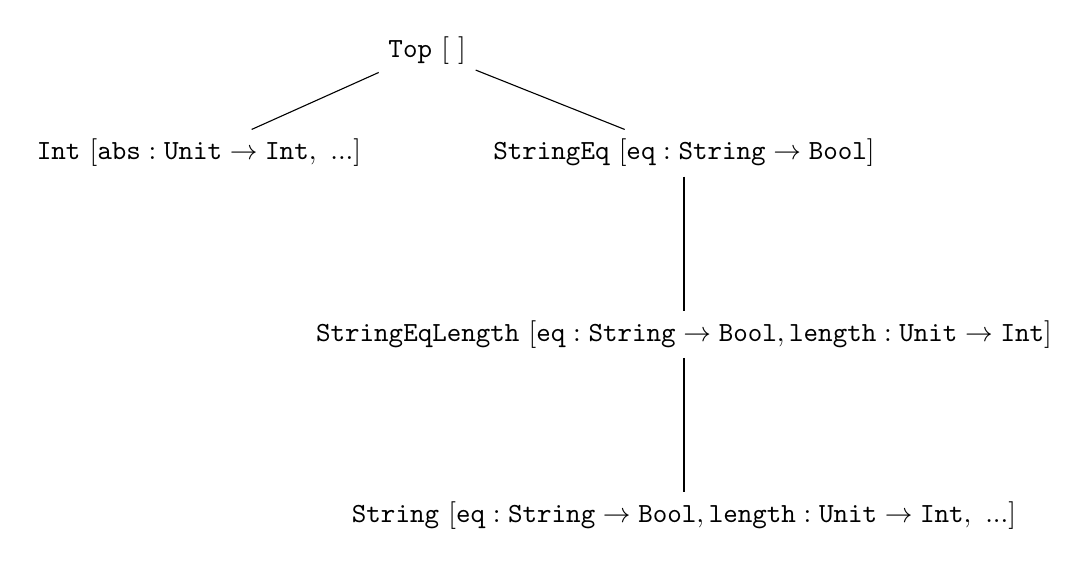
\begin{tikzpicture}[node distance=2.3cm]
			\node(Top) 												{\texttt{Top} $\triangleq [\ ]$};
			\node(StringEq)		[below right=0.7cm and 0.1cm of Top]			{\texttt{StringEq} $\triangleq [\mathtt{eq} : \mathtt{String} \rightarrow \mathtt{Bool}]$};
			\node(StringEqLength)      [below of=StringEq]       {\texttt{StringEqLength} $\triangleq [\mathtt{eq} : \mathtt{String} \rightarrow \mathtt{Bool}, \mathtt{length} : \mathtt{Unit} \rightarrow \mathtt{Int}]$};
			\node(String)				[below of=StringEqLength]       {\texttt{String} $\triangleq [\mathtt{eq} : \mathtt{String} \rightarrow \mathtt{Bool}, \mathtt{length} : \mathtt{Unit} \rightarrow \mathtt{Int},\ ...]$};
			\node(int)					[below left=0.7cm and 0.1cm of Top] 			{\texttt{Int} $\triangleq [\mathtt{abs} : \mathtt{Unit} \rightarrow \mathtt{Int},\ ...]$};
			\draw(Top)      -- (StringEq);
			\draw(Top)      -- (int);
			\draw(StringEq)      -- (StringEqLength);
			\draw(StringEqLength)      -- (String);
		\end{tikzpicture}
		\caption{retículo de subtipos}
    \label{l1}
	\end{figure}

Los métodos declarados en la faceta pública también poseen tipos de dos facetas en sus firmas. Así, el tipo \texttt{StringEq} visto anteriormente se define como $\mathtt{StringEq} \triangleq [\mathtt{eq} : \mathtt{String}$\texttt{<}$\mathtt{String} \rightarrow \mathtt{Bool}$\texttt{<}$\mathtt{Bool}]$.

Existen dos reglas principales para comprobar que un programa con tipos de dos facetas se encuentra bien tipado. Consideremos el siguiente ejemplo, en donde $\mathtt{StringHashEq} \triangleq [\mathtt{hash} : \mathtt{Unit}$\texttt{<}$\mathtt{Unit} \rightarrow \mathtt{String}$\texttt{<}$\mathtt{StringEq}]$.

\begin{ej} \ \\
  \normalfont
  \label{ej2-6}
\begin{lstlisting}
  String<StringEq getHash(String<StringHashEq password) {
  	return password.hash();
  }
\end{lstlisting}
\end{ej}

En el ejemplo \ref{ej2-6}, el valor de retorno de la invocación al método \texttt{hash} sobre el parámetro \texttt{password}, tiene faceta pública \texttt{StringEq}, debido a que fue declarado de esta forma en la faceta pública \texttt{StringHashEq}. A esta regla se le llama \texttt{TmD}.

Ahora consideremos el siguiente ejemplo, en donde se cambia la faceta pública del parámetro \texttt{password} del ejemplo \ref{ej2-6} por \texttt{StringEq}.

\begin{ej} \ \\
  \normalfont
  \label{ej2-7}
\begin{lstlisting}
  String<Top getHash(String<StringEq password) {
  	return password.hash();
  }
\end{lstlisting}
\end{ej}

En el ejemplo \ref{ej2-7} se realiza una invocación al método \texttt{hash} sobre el parámetro \texttt{password}, que declara una faceta pública que no autoriza la operación. Cuando esto sucede, la faceta pública de retorno de la invocación es \texttt{Top}. A esta regla se le llama \texttt{TmH}.

La propiedad de seguridad que se demuestra para el sistema de tipos de la desclasificación basada en tipos es una forma de no-interferencia con políticas de desclasificación, denominada no-interferencia relajada (\emph{Relaxed noninterference}). Un lenguaje de seguridad que cumple con esta propiedad, garantiza que la información confidencial solo puede fluir hacia canales públicos de forma controlada, por medio de las políticas de desclasificación.

\section{Inferencia de tipos} \label{inference}
En la sección anterior se revisaron los conceptos relacionados a control de flujo de información, que sirven para comprender el trabajo de la desclasificación basada en tipos. En esta sección se revisan los conceptos relacionados a inferencia de tipos, necesarios para comprender la propuesta de esta memoria.

La inferencia de tipos es el proceso de determinar el tipo de las expresiones en un programa, basado en cómo son usadas. Tener un mecanismo de inferencia en un lenguaje de programación puede ser muy útil, debido a que da la posibilidad al programador de omitir las declaraciones de tipo para algunos identificadores, y mantener los beneficios de un lenguaje estáticamente tipado.

Para ilustrar los conceptos importantes de inferencia, consideremos un lenguaje sencillo con funciones y operaciones aritméticas sobre enteros, cuya sintaxis se muestra en el siguiente ejemplo.
\vspace{0.8em}
\begin{ej}
  \normalfont
  \label{ej2-8}
\begin{lstlisting}
  let g = (x) => x + 5;
\end{lstlisting}
\end{ej}

En el ejemplo \ref{ej2-8}, se asigna a \texttt{g} una función que retorna la suma entre \texttt{x} y \texttt{5}. Notar que no se anotó el tipo de los identificadores \texttt{g} y \texttt{x}.

En la etapa de tipar un programa (\emph{type checking}), los sistemas de inferencia asignan una variable de tipo a cada expresión sin un tipo conocido, y un tipo concreto\footnote{Un tipo concreto no tiene variables de tipo} (por ejemplo, \texttt{int}) a cada expresión con tipo conocido. Además, generan un conjunto de restricciones que se deben cumplir para que cada expresión esté bien tipada.
\clearpage

Una restricción representa una relación entre dos tipos. Esta relación puede ser de igualdad o de subtipos. El uso de restricciones permite presentar un algoritmo de inferencia de forma modular, como una fase de generación de restricciones, y una fase de resolución de restricciones.

La figura \ref{tabla1} muestra la asignación de tipos a cada una de las expresiones del ejemplo \ref{ej2-8}, y las restricciones que se generan.


\begin{figure}[ht]
  \centering
  \ttfamily
  \begin{tabular}{c c c}
    Expresión & Tipo & Restricciones\\
    \hline
    (x) =>\ x + 5 & X & $\mathtt{X = Y \rightarrow Z}$\\
    x & Y & -\\
    x + 5 & Z & Y = int, Z = int\\
    + & $\mathtt{(int,int) \rightarrow int}$ & -\\
    x & Y & -\\
    5 & int & -\\
  \end{tabular}
  \caption{Etapa de \emph{type checking}}
  \label{tabla1}
\end{figure}

En el ejemplo \ref{ej2-8}, las restricciones generadas representan igualdad entre dos tipos. Las siguientes observaciones permiten derivar conjunto de restricciones del programa.

\begin{enumerate}
  \item \texttt{(x) =>\ x + 5} es una función anónima que debe tener tipo $\mathtt{Y \rightarrow Z}$, donde \texttt{Y} es el tipo del parámetro y \texttt{Z} es el tipo del cuerpo.
  \item \texttt{x + 5} es una aplicación de la función suma, por lo que su tipo debe coincidir con el tipo de retorno de la función. Además, el tipo de los argumentos debe coincidir con el tipo de los parámetros de la función.
\end{enumerate}

Sintetizando, el conjunto de restricciones generado es el siguiente:

\begin{itemize}
  \item $\mathtt{X = Y \rightarrow Z}$
  \item \texttt{Y = int}
  \item \texttt{Z = int}
\end{itemize}

Una vez que se genera el conjunto de restricciones sobre el programa, se procede a encontrar una solución para las variables de tipo del conjunto. Cuando las restricciones representan relaciones de igualdad, se utiliza el algoritmo de unificación de Damas-Milner~\cite{damasmilner}. Este algoritmo genera un diccionario de variables de tipo a tipos concretos, mediante substituciones. La figura \ref{tabla2} muestra la solución esperada del ejemplo \ref{ej2-8}.

\begin{figure}[ht]
  \centering
  \ttfamily
  \begin{tabular}{c c}
    Variable de tipo & Tipo concreto \\
    \hline
    X & $\mathtt{int \rightarrow int}$  \\
    Y & int \\
    Z & int \\
  \end{tabular}
  \caption{Solución del conjunto de restricciones}
  \label{tabla2}
\end{figure}

\clearpage
Desafortunadamente, el algoritmo de unificación de Damas-Milner no funciona cuando las restricciones representan una relación de subtipos. Consideremos una extensión del lenguaje anterior,  en donde se introducen los tipos \texttt{num} y \texttt{float}, donde se cumple \texttt{float <: num} y \texttt{int <: num}. En el ejemplo \ref{ej2-9} se muestran dos instrucciones de asignación.
\vspace{0.8em}
\begin{ej}
  \normalfont
  \label{ej2-9}
\begin{lstlisting}
  let f = 4;
                ...
                f = 1.5;
\end{lstlisting}
\end{ej}

En el ejemplo \ref{ej2-9}, se asigna la variable de tipo \texttt{X} al identificador \texttt{f}. Las restricciones que se generan para las instrucciones de asignación son:

\begin{itemize}
  \item \texttt{int <: X}
  \item \texttt{float <: X}
\end{itemize}

%Cardelli~\cite{cardelli}

Para resolver este tipo de relaciones, se considera la relación de orden parcial entre los tipos, inducida por la relación de subtipos, que se muestra en la figura \ref{subt1}.

\begin{figure}[ht]
  \centering
  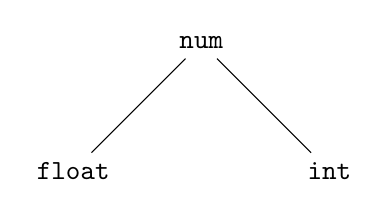
\begin{tikzpicture}[node distance=2.3cm]
    \node(num) 												{\texttt{num}};
    \node(int)		[below right of=num]			{\texttt{int}};
    \node(float)					[below left of=num] 			{\texttt{float}};
    \draw (num)      -- (int);
    \draw (num)      -- (float);
  \end{tikzpicture}
  \caption{Orden parcial entre los tipos}
  \label{subt1}
\end{figure}

Un orden parcial admite las operaciones \texttt{meet} y \texttt{join}, que corresponden a la máxima cota inferior (ínfimo) y a la mínima cota superior (supremo) entre dos tipos, respectivamente. Estas operaciones tienen solución si todo par de tipos en el orden parcial tiene un único supremo e ínfimo, lo que se define como retículo. En la figura \ref{subt1}, se debe agregar el tipo \texttt{Bot} para que el orden parcial sea un retículo.

Luego, se introducen los tipos $\mathtt{t_1 \sqcap t_2}$ y $\mathtt{t_1 \sqcup t_2}$, que representan a las operaciones \texttt{meet} y \texttt{join} entre dos tipos, respectivamente.

En la fase de resolución de restricciones, se aplican las reglas de la proposición \ref{teo1} para generar los tipos correspondientes. Luego, cuando los tipos $\sqcap$ y $\sqcup$ relacionan tipos concretos, se puede materializar la operación sobre el retículo.

%Pese a que Cardelli no considera una inferencia basada en constraints, se puede aplicar este enfoque para la resolución de constraints de subtyping. En efecto, Pottier~\cite{pottier:inria-00073205} y Sekiguchi~\cite{sekiguchi} presentan sistemas de inferencia basados en constraints, con tipos equivalentes a los \texttt{meet} y \texttt{join} de Cardelli.

\begin{prop} \label{teo1} \normalfont Si \texttt{x}, \texttt{y} y \texttt{z} pertenecen a una retículo de subtipos, se cumple lo siguiente: \\
  \begin{itemize}
    \item \texttt{x <: y}, \texttt{x <: z} $\implies$ $\mathtt{x <: y \sqcap z}$
    \item \texttt{y <: x}, \texttt{z <: x} $\implies$ $\mathtt{y \sqcup z <: x}$
  \end{itemize}
\end{prop}

En el ejemplo \ref{ej2-9}, las restricciones generadas se reducen con la aplicación de la proposición \ref{teo1}, lo que da como resultado la restricción $\mathtt{int\sqcup float <: X}$. Como \texttt{int} y \texttt{float} son tipos concretos, se puede materializar la operación \texttt{join}, lo que da como resultado \texttt{num}.

Finalmente, como la restricción \texttt{num <: X} solo admite una solución para \texttt{X}, se resuelve que \texttt{X} tiene tipo \texttt{num}.

\subsection*{Notas}

En el ejemplo \ref{ej2-9}, la relación de subtipos es nominal. En una relación de subtipos nominal, el retículo de subtipos se define por la jerarquía que conforman los tipos, la cual fue definida explícitamente por el programador o el lenguaje de programación. El ejemplo \ref{ej2-10} muestra una declaración explícita de la jerarquía de los tipos del ejemplo \ref{ej2-9}.

\begin{ej} \ \\
  \normalfont
  \label{ej2-10}
\begin{lstlisting}
  class Num {
    Num +(Num n2);
    Num *(Num n2);
  }

  class Int extends Num { }

  class Float extends Num {
    Int ceil();
  }
\end{lstlisting}
\end{ej}

Cuando una relación de subtipos es estructural, el retículo de subtipos se define por la forma que tienen los tipos. El ejemplo \ref{ej2-11} muestra la declaración de las clases que definen a los tipos del ejemplo \ref{ej2-9}. En este caso, \texttt{Int} y \texttt{Float} son subtipos de \texttt{Num} porque tienen al menos los mismos métodos que tiene \texttt{Num}.

\begin{ej} \ \\
  \normalfont
  \label{ej2-11}
\begin{lstlisting}
  class Num {
    Num +(Num n2);
    Num *(Num n2);
  }

  class Int {
    Int +(Num n2);
    Int *(Num n2);
  }

  class Float {
    Float +(Num n2);
    Float *(Num n2);
    Int ceil();
  }
\end{lstlisting}
\end{ej}

%Los tipos $\sqcap$ y $\sqcup$ fueron utilizados por vez primera en un algoritmo de inferencia por Cardelli~\cite{cardelli}.

% Teniendo en cuenta que los distintos sistemas de inferencia propuestos a lo largo del tiempo comparten características, Odersky \textit{et al.}~\cite{odersky} propusieron el framework \texttt{HM(X)}, que entrega un algoritmo de inferencia genérico para un sistema de tipos basado en constraints que cumpla ciertas condiciones.

% Utilizando el framework \texttt{HM(X)}, Pottier y Simonet~\cite{Pottier} presentaron un análisis de control de flujo con inferencia de tipos de seguridad, que hereda todas las buenas propiedades de \texttt{HM(X)}.

\chapter{Propuesta}

En este trabajo se propone realizar la implementación en Dart de un sistema de inferencia de facetas de declasificación, que incluya el análisis de \textit{Type-based Relaxed Noninterference}, mediante la realización de un plugin para entornos de desarrollo integrado (IDE). En este capítulo se detallan los problemas de inferencia a resolver, las estrategias utilizadas para resolverlos, los cambios al trabajo original y el subconjunto del lenguaje soportado.

\section{Problema de inferencia}
Se discute el problema de inferencia a resolver y ejemplos de lo que se busca del sistema a implementar.

\section{Consideraciones de diseño}
Se discuten las alternativas disponibles respecto a la decisión sobre las facetas de métodos que pertenecen al core del lenguaje, y por qué Bot -> Bot es la escogida. Explicar que de todas formas sería un parámetro configurable de la herramienta.

\section{Generación de constraints de subtyping}
Se muestra en palabras la generación de constraints para las distintas expresiones.
\subsection{Declaración de métodos}
\subsection{Llamadas a métodos}
\subsubsection{Retorno}
\subsubsection{Argumentos}
\subsubsection{Encadenamiento de llamados}
\subsection{Expresión de retorno}
\subsection{Declaración y asignación a variables}
\subsection{Expresiones condicionales}



\section{Resolución de constraints}

\subsection{Simplificación y eliminación de constraints}
\subsection{Agrupación de constraints}
\subsubsection{Join}
\subsubsection{Meet}
\subsection{Unificación y substitución}


\section{Extensión de propuesta teórica}
Mostrar los cambios y extensiones necesarias al trabajo de type-based declassification para ajustarse a un lenguaje como Dart, y el subconjunto de Dart soportado.

\section{Interacción con el usuario}
Cuál es la interacción con el usuario deseada.

\chapter{Implementación}
En esta sección se detalla la implementación de este trabajo, que se dividió en dos componentes principales. Primero, se implementó un sistema de inferencia para type-based declassification. Segundo, se elaboró un plugin para editores de texto que integra el resultado de la inferencia.

\section{Lenguaje Dart}
Dart es un lenguaje de programación de propósito general, orientado a objetos y de código abierto desarrollado por Google. Es usado para construir aplicaciones web, móviles y dispositivos IoT (Internet of Things).

La implementación de este trabajo fue realizada en Dart, debido a que proporciona las herramientas necesarias para realizar el análisis requerido, como el AST (Abstract Syntax Tree) resuelto con la información completa de tipos. Además, los investigadores que realizaron el trabajo de \textit{type-based declassification} estudian este lenguaje como parte de un proyecto de investigación mayor en el área de seguridad.

\subsection{Dart Analyzer}
\textit{Dart Analyer} es una herramienta incluida en Dart, que permite realizar análisis estático de código Dart. Entre otros servicios, esta herramienta permite obtener un AST (Abstract Syntax Tree) dado un código Dart. Dicho AST contiene la información relevante del programa, incluyendo el resultado del análisis de tipos.

Análisis personalizados de programas en Dart pueden ser realizados usando la información del AST. En efecto, Dart Analyzer utiliza el patrón Visitor para incorporar un nuevo análisis sobre el AST.

\subsection{Analyzer Plugin}
La herramienta \textit{Analyzer Plugin} sirve para integrar un análisis personalizado sobre el AST generado por \textit{Dart Analyzer}, con los IDE que tengan soporte para servidores de análisis estático de Dart, como IntelliJ, Eclipse, Atom, entre otros. Con esta librería es posible mostrar errores, \textit{warnings}, sugerencias de edición, sugerencias de navegación  y resaltado de sintaxis.

\section{Implementación de sistema de inferencia}

\subsection{Representación de facetas de desclasificación}
Para declarar las facetas de desclasificación, se usarán las anotaciones de Dart. Por ejemplo, \texttt{@S("Top") bool check(@S("StringCompareTo") String password);} es una declaración de un método de Dart anotado con facetas de desclasificación.

La definición de las facetas de desclasificación se hace mediante clases abstractas de Dart. Por ejemplo, la faceta \texttt{StringCompareTo} se define mediante la clase abstracta del mismo nombre:

\begin{lstlisting}
  abstract class StringCompareTo {
    int compareTo(String other);
  }
\end{lstlisting}

Antes de la generación de constraints sobre un archivo, se realiza una etapa de \textit{parsing} de facetas de desclasificación, en donde se leen las clases abstractas del archivo. Esto se implementa mediante el \textit{visitor} \texttt{DeclaredFacetVisitor}, que se muestra en el diagrama de la figura XXX. Las facetas de desclasificación procesadas se almacenan en el diccionario \texttt{declaredStore}, en donde se asocia el nombre de la faceta con su tipo de objeto correspondiente.

\subsection{Fase de generación de constraints}
Una vez que se procesan las facetas de desclasificación, se procede a la generación de constraints. Esto se realiza implementando varios \textit{visitors} mostrados en el diagrama de la figura XXX.

La clase encargada de procesar un archivo es \texttt{CompilationUnitVisitor}, en donde se procesa cada clase declarada en el archivo. Mediante el \textit{visitor} \texttt{ClassMemberVisitor}, se procesa cada método, campo y constructor de cada clase. Finalmente, el \textit{visitor} implementado para procesar el cuerpo de cada miembro es \texttt{BlockVisitor}, en donde se procesa cada expresión relevante para el algoritmo de generación de constraints de la sección \ref{propuestaGen}.

La clase \texttt{Store} es la encargada de la generación de variables de tipo, y el almacenamiento en diccionarios del tipo de las expresiones. Cada visita a los nodos del AST puede agregar constraints al set de constraints, y agregar o actualizar elementos en el store. Ambos se muestran en el diagrama YYY.

En la fase de generación de constraints se pueden generar warnings, al declarar una faceta no definida. Esto se recolecta mediante un \texttt{ErrorCollector}, el cual será utilizado para el despliegue de la información mediante el plugin.

\subsection{Fase de resolución de constraints}

\subsubsection{Recolección de errores}

\subsection{Testing}
Cómo se testea la inferencia.

\section{Implementación de plugin}

\subsection{Diagrama de componentes y descripción general}
Explicar funcionamiento general e integración con sistema de inferencia.

\subsection{Configuración inicial}
Uso de la herramienta y creación del archivo sec.dart en primera ejecución del análisis.

\subsection{Tipos de errores e información}

\chapter{Validación}

\section{Programando con facetas públicas}
Poseer un sistema de inferencia en conjunto con un plugin para IDEs tiene múltiples beneficios. Primero, evita la anotación de facetas públicas en identificadores no relevantes para el análisis. Segundo, provee comodidad al momento de programar, ya que se obtienen en tiempo real los resultados de la inferencia, sin tener que re-ejecutar un análisis. Por último, aumenta la escalabilidad de los sistemas, ya que el costo de refactorizar código anotado es mayor al costo de refactorizar código no anotado.

A continuación, se muestran algunas capturas de pantalla que ejemplifican la interacción entre el plugin y el programador.

La figura \ref{screen1} ilustra la integración de los errores del plugin con los errores de Dart, en la misma ventana del IDE.

\begin{figure}[ht]
  \centering
  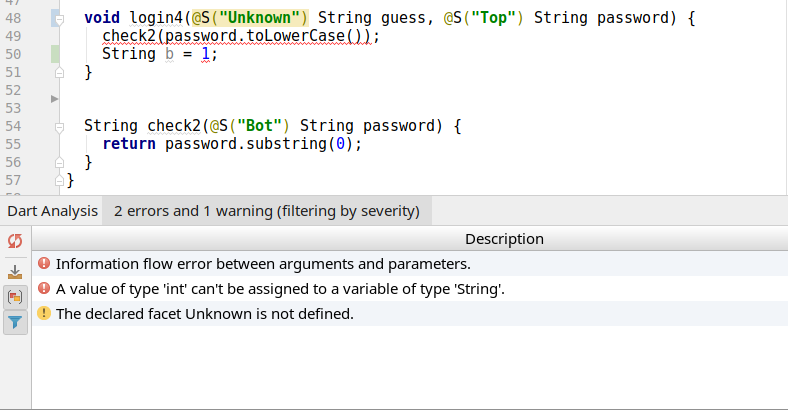
\includegraphics[width=0.8\textwidth]{imagenes/screen1.png}
  \caption{Errores integrados con errores de Dart}
  \label{screen1}
\end{figure}
\clearpage

La figura \ref{screen2} muestra la información inferida al ubicar el cursor sobre un identificador sin faceta pública definida.

\begin{figure}[ht]
  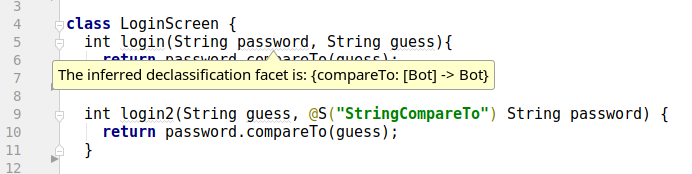
\includegraphics[width=\textwidth]{imagenes/facetinfo.png}
  \caption{Faceta pública inferida}
  \label{screen2}
\end{figure}


La figura \ref{screen3} muestra un error generado por un flujo no permitido.

\begin{figure}[ht]
  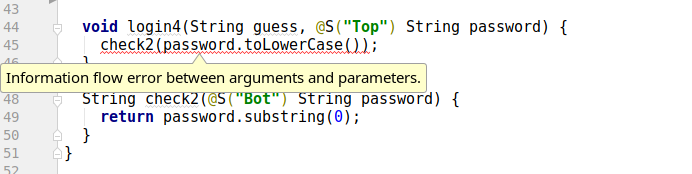
\includegraphics[width=\textwidth]{imagenes/flow.png}
  \caption{Error de flujo de información}
  \label{screen3}
\end{figure}

La figura \ref{screen4} muestra un error generado por la declaración de una faceta pública no definida.

\begin{figure}[ht]
  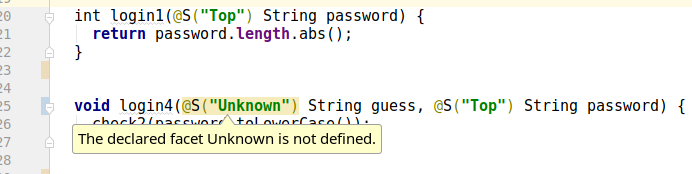
\includegraphics[width=\textwidth]{imagenes/undefined.png}
  \caption{Warning ante faceta pública no definida}
  \label{screen4}
\end{figure}
\clearpage
La figura \ref{screen5} muestra un identificador cuya faceta pública no pudo ser inferida con precisión, debido a que cualquier faceta genera un programa bien tipado.

\begin{figure}[ht]
  
\includegraphics[width=\textwidth]{imagenes/any.png}
  \caption{Toda faceta pública genera un programa bien tipado}
  \label{screen5}
\end{figure}

\section{Batería de tests}
En conjunto con uno de los autores de type-based declassification, se validaron una serie de tests unitarios que ponen a prueba el cumplimiento de las reglas del sistema de tipos.

Además de proveer una forma de validación de este trabajo, los tests unitarios sirvieron como guía para la implementación de las distintas componentes.

Para escribir los tests se utilizó la librería estándar de testing en Dart.

\section{Repositorio de prueba}
Para demostrar el uso del análisis en un ejemplo realista, se creó un pequeño sistema de login web, programado con facetas públicas de type-based declassification. El código se encuentra en un repositorio de GitHub~\cite{repotest}.

En este ejemplo se pudo constatar la utilidad del sistema de inferencia. De las 20 declaraciones de identificadores del código, solo 6 de ellas fueron anotadas con facetas públicas, y el resto fue inferido de acuerdo a las reglas del sistema de tipos.

\begin{conclusion}

	Type-based declassification muestra una conexión entre las relaciones de subtyping de un lenguaje orientado a objetos, y las relaciones de orden que conforman los tipos de seguridad, para proponer un sistema de tipos que cumple una versión relajada de noninterference. Con esta propuesta, Cruz \textit{et al.} abordan parcialmente el desafió de integrar los modelos de control de flujo de información con infraestructuras existentes. Este trabajo materializa aquella propuesta, con una implementación para un subconjunto del lenguaje Dart, en conjunto con un sistema de inferencia y un plugin para editores.

	A pesar del foco de seguridad que tiene un trabajo de estas características, la formulación del problema de inferencia y el uso del plugin para integrar los resultados fueron concebidos teniendo al programador en mente, para facilitarle el trabajo y mejorar su experiencia programando, entre otros beneficios. Esta experiencia puede mejorar aún más, agregando nuevas características al plugin.

	\section*{Trabajo futuro}

	\paragraph{Formalización de inferencia.}En este trabajo se implmentó un sistema de inferencia sin demostrar que la extensión necesaria al sistema de tipos de type-based declassification preserva las propiedades del trabajo original, como son \emph{type safety} y relaxed noninterference. En este sentido, es deseable la formalización de la inferencia de tipos de dos facetas, antes de realizar cualquier extensión a este trabajo, cuyo objetivo fue demostrar el uso práctico del enfoque propuesto por Cruz \textit{et al.}

	\paragraph{Extensión al subconjunto soportado.}Este trabajo soporta un subconjunto pequeño del lenguaje Dart, lo que no permite probarlo en aplicaciones reales de mayor envergadura. Soportar características avanzadas del lenguaje, e implementar la herramienta en otros lenguajes de programación, permitiría posicionar a la herramienta como una alternativa competente de análisis de control de flujo para aplicaciones en producción.

	\paragraph{Características del plugin.}El plugin implementado en este trabajo solo muestra los resultados de la inferencia, pero no permite al programador tomar acciones automáticas al respecto. Por ejemplo, es posible asistir al usuario en la definición de una faceta pública que ha sido declarada, navegar al lugar donde se define una faceta pública al ubicarse en la faceta declarada, definir y declarar una faceta pública basándose en el resultado de la inferencia, entre otros.



\end{conclusion}


% \input{glosario.tex} % opcional

\bibliographystyle{plain}
\bibliography{bibliografia}

% \input{anexo_apendices.tex} % opcionales

\end{document}
